\chapter{Macro-programming}\label{chap:macro-programming}
\minitoc% Creating an actual minitoc
Macroprogramming, as a paradigm, 
 has emerged as a pivotal approach in the realm of distributed systems. 
%
It offers a unique perspective, 
 allowing developers to express the \emph{macroscopic behaviour} of a collective system using a singular program.
% 
This chapter delves into the intricacies of macroprogramming, 
 its historical evolution, and its significance in the modern computational landscape, 
 leading to aggregate computing -- a novel macro-programming approach for Cyber-Physical Swarms.

\begin{figure}
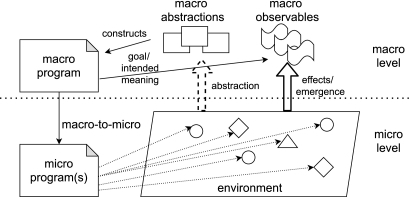
\includegraphics[width=\textwidth]{chapters/img/macro-programming.jpg}
\caption{Overview of macroprogramming}\label{macro:fig:macro-programming}
\end{figure}
\section{The Essence of Macroprogramming}
Macroprogramming  emphasizes the overarching behaviour of a system, abstracting the intricacies of individual components. 
 This abstraction is crucial for systems where the collective behaviour is more significant than the sum of its parts.

The primary motivation behind macroprogramming 
 is to simplify the design and development of complex systems. 
 By providing a higher-level perspective, 
 it allows developers to address system-wide concerns without getting bogged down by the details of individual components. 
 This not only streamlines the development process but also ensures that the system's behaviour is \emph{consistent} and \emph{predictable}.

In essence, macroprogramming is about seeing the \emph{forest} for the \emph{trees}. 
 It recognizes that while individual components (or trees) are essential,
 understanding and managing their collective behaviour (or the forest) is of paramount importance. 
This perspective is particularly relevant in today's interconnected world, 
 where systems often comprise numerous components that need to work in harmony.

Furthermore, macroprogramming leverages macro-level abstractions, 
 such as \emph{collective states}, \emph{groups}, or \emph{spatiotemporal} patterns. 
 These abstractions provide a structured way to think about and design systems, ensuring that they are both \emph{robust} and \emph{adaptable}. 
By focusing on these higher-level abstractions, 
 macroprogramming allows for a more intuitive and efficient approach to system design, 
 making it an indispensable tool in the modern developer's toolkit.
\Cref{macro:fig:macro-programming} provides an overview of the idea behind this paradigm.

Diving deeper into the terminology, 
 terms like ``system programming'', ``centralized programming'', and ``high-level programming'' 
 have been used in various contexts, leading to potential confusion. 
% 
Among these, domain-specific terms like ``global-level programming'', ``swarm programming'', and 
 ``aggregate programming'' stand out. 
%
These terms reflect the diverse perspectives from which macroprogramming can be approached, 
 emphasizing the need for a unified framework that can consolidate these diverse viewpoints. 
%
Such a framework would not only provide clarity but also pave the way for innovative solutions in the realm of systemic behaviour modelling.

\section{Conceptual Framework}

\subsection{Preliminaries}
Macroprogramming addresses the challenge of programming the behaviour of a computational system \( S \), composed of multiple computational entities. Given two entities \( A \) and \( B \) within this system, there are three primary modes to influence their behaviour to promote properties ascribable to \( S \):
\begin{enumerate}
    \item Altering their context, indirectly influencing them. For instance, a change in sensor \( A \) might subsequently affect \( B \).
    \item Interaction, such as triggering their behaviour. If \( A \) is an actuator, its actions might influence \( B \).
    \item Setting their behaviour to produce certain global outcomes when activated.
\end{enumerate}
The term "program" refers to an abstract description executable by a computational entity. Modes (1) and (2) allow an external entity \( C \) to influence \( A \) or \( B \), and consequently \( S \).

\subsection{Macroprogramming: Definition and Basic Concepts}
Macroprogramming is defined as an abstract paradigm for programming the macroscopic behaviour of systems of computational entities. As a paradigm, it's an approach rooted in a mathematical theory or a set of coherent principles. The foundational principles of macroprogramming include:
\begin{itemize}
    \item Micro-macro distinction: Recognizing two primary system levels - macro (global structures) and micro (computational entities).
    \item Macroscopic perspective: Focusing on the system's macroscopic aspects, considering micro-level entities from a global perspective.
    \item Macroprogram: The result of macroprogramming, a program executed by the system adopting the macroscopic perspective.
    \item Macro-to-micro mapping: Implementing how a macroprogram is executed by the system, defining a logic to map macro instructions to micro-level behaviors.
\end{itemize}

\subsubsection{On Micro-Macro and Local-Global Distinction}
The micro-macro distinction is prevalent in various scientific areas, distinguishing smaller elements from larger ones. For programming, a system can be defined based on a boundary condition, distinguishing between the micro and macro dimensions. The goal of macroprogramming is closely tied to the concept of emergence, analysing the relationships between microscopic and macroscopic states.

\subsubsection{On Collectives}
Macroprogramming often targets collectives, groups of similar entities sharing common traits or goals. While heterogeneous collectives exist, they tend to complicate macroprogramming by emphasizing individual perspectives or widening the macro-to-micro gap.

\subsubsection{On Declaratively}
Declarativity is a hallmark of macroprogramming, focusing on the computation's goal rather than its method. This approach abstracts away specific computational aspects, offering high-level abstractions tailored to specific application domains, often resulting in Domain-Specific Languages (DSLs).

\subsection{Historical Evolution and Context}

The historical roots of macroprogramming can be traced back to the pioneering work of Newton and Welsh in 2004. 
 Their research laid the foundation for the application of macroprogramming in the domain of Wireless Sensor Networks (WSNs). 
 These networks, characterized by embedded units equipped with processing, communication, and sensing capabilities, presented unique challenges that necessitated a macroscopic view for effective data processing and logic description. 
The emphasis was on capturing the collective behaviour of these sensor nodes, 
 ensuring efficient data aggregation, processing, and communication.

WSNs were among the first systems that required a departure from traditional programming paradigms. 
 Given the distributed nature of these networks and the limited resources of individual sensor nodes, 
 there was a pressing need to optimize both computation and communication. 
 Macroprogramming emerged as a solution, allowing developers to focus on the overall behaviour of the network rather than the intricacies of individual nodes.

As technology evolved, so did the applications of macroprogramming. 
 The rise of the Internet of Things (IoT) in the subsequent years brought forth a plethora of interconnected devices, each with its own set of capabilities and functions. 
 The complexity of these systems further underscored the importance of a macroscopic approach. Macroprogramming principles were adapted and refined to cater to the diverse requirements of IoT ecosystems.

Furthermore, the emergence of Cyber-Physical Systems (CPSs) and spatial computing introduced new challenges and opportunities for macroprogramming. 
 These systems, which integrate computational processes with physical entities, demanded a holistic approach to ensure seamless interaction and coordination. 
 Macroprogramming, with its emphasis on collective behaviour and high-level abstractions, proved to be an invaluable tool in this context.

Over the years, the principles of macroprogramming have been enriched by interdisciplinary research, drawing insights from fields such as distributed systems, artificial intelligence, and network theory. 
 This confluence of ideas has shaped the evolution of macroprogramming, making it a dynamic and ever-evolving field that continues to adapt to the changing technological landscape.

\section{Aggregate computing}
\subsection{Field Calculus}
\subsection{Motivating examples}
\subsection{Aggregate programming}
\section{Wrap up}

Macroprogramming, with its focus on the macroscopic behaviour of systems, 
 has proven to be an invaluable tool in the computational world. 
%
From its early applications in WSNs to its modern-day relevance in IoT and CPSs, 
 it has consistently demonstrated its utility. 
As we move towards an increasingly interconnected world, 
 the principles of macroprogramming will undoubtedly play a pivotal role in shaping the future of computational systems.

 \printbibliography